\begin{figure}[htbp]
    \centering
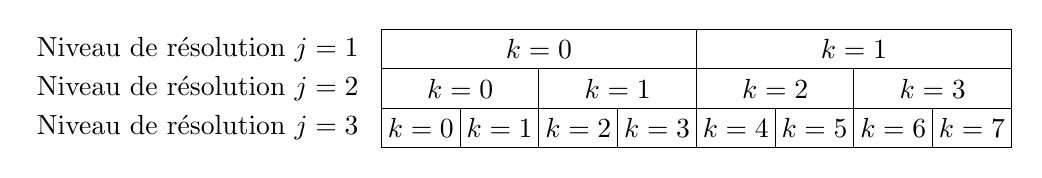
\begin{tikzpicture}


\node[anchor=west] at (-8.5, -.25) {Niveau de résolution $j=3$};
\node[anchor=west] at (-8.5, .25) {Niveau de résolution $j=2$};
\node[anchor=west] at (-8.5, .75) {Niveau de résolution $j=1$};
% Niveau j-1

\draw (-4,.5) rectangle (0,1);
\draw (0,.5) rectangle (4,1);

    % Niveau j
\draw (-4,0) rectangle (-2,.5);
\draw (-2,0) rectangle (0,.5);
\draw (0,0) rectangle (2,.5);
\draw (2,0) rectangle (4,.5);
%\node at (1,1.75) {$k=2$};

% Niveau j+1

\draw (-4,-.5) rectangle (-3,0);
\draw (-3,-.5) rectangle (-2,0);
\draw (-2,-.5) rectangle (-1,0);
\draw (-1,-.5) rectangle (0,0);
\draw (0,-.5) rectangle (1,0);
\draw (1,-.5) rectangle (2,0);
\draw (2,-.5) rectangle (3,0);
\draw (3,-.5) rectangle (4,0);

% Relations
\node at (-2, .75) {$k=0$};
\node at (+2, .75) {$k=1$};

\node at (-3, .25) {$k=0$};
\node at (-1, .25) {$k=1$};
\node at (+1, .25) {$k=2$};
\node at (+3, .25) {$k=3$};

\node at (-3.5, -.25) {$k=0$};
\node at (-2.5, -.25) {$k=1$};
\node at (-1.5, -.25) {$k=2$};
\node at (-0.5, -.25) {$k=3$};

\node at (+0.5, -.25) {$k=4$};
\node at (+1.5, -.25) {$k=5$};
\node at (+2.5, -.25) {$k=6$};
\node at (+3.5, -.25) {$k=7$};


\end{tikzpicture}
\caption{Exemple de grille dyadique}
\label{fig:schema_sdyadique}
\end{figure}